% Options for packages loaded elsewhere
\PassOptionsToPackage{unicode}{hyperref}
\PassOptionsToPackage{hyphens}{url}
\PassOptionsToPackage{dvipsnames,svgnames,x11names}{xcolor}
%
\documentclass[
  letterpaper,
  DIV=11,
  numbers=noendperiod]{scrartcl}

\usepackage{amsmath,amssymb}
\usepackage{iftex}
\ifPDFTeX
  \usepackage[T1]{fontenc}
  \usepackage[utf8]{inputenc}
  \usepackage{textcomp} % provide euro and other symbols
\else % if luatex or xetex
  \usepackage{unicode-math}
  \defaultfontfeatures{Scale=MatchLowercase}
  \defaultfontfeatures[\rmfamily]{Ligatures=TeX,Scale=1}
\fi
\usepackage{lmodern}
\ifPDFTeX\else  
    % xetex/luatex font selection
\fi
% Use upquote if available, for straight quotes in verbatim environments
\IfFileExists{upquote.sty}{\usepackage{upquote}}{}
\IfFileExists{microtype.sty}{% use microtype if available
  \usepackage[]{microtype}
  \UseMicrotypeSet[protrusion]{basicmath} % disable protrusion for tt fonts
}{}
\makeatletter
\@ifundefined{KOMAClassName}{% if non-KOMA class
  \IfFileExists{parskip.sty}{%
    \usepackage{parskip}
  }{% else
    \setlength{\parindent}{0pt}
    \setlength{\parskip}{6pt plus 2pt minus 1pt}}
}{% if KOMA class
  \KOMAoptions{parskip=half}}
\makeatother
\usepackage{xcolor}
\setlength{\emergencystretch}{3em} % prevent overfull lines
\setcounter{secnumdepth}{5}
% Make \paragraph and \subparagraph free-standing
\makeatletter
\ifx\paragraph\undefined\else
  \let\oldparagraph\paragraph
  \renewcommand{\paragraph}{
    \@ifstar
      \xxxParagraphStar
      \xxxParagraphNoStar
  }
  \newcommand{\xxxParagraphStar}[1]{\oldparagraph*{#1}\mbox{}}
  \newcommand{\xxxParagraphNoStar}[1]{\oldparagraph{#1}\mbox{}}
\fi
\ifx\subparagraph\undefined\else
  \let\oldsubparagraph\subparagraph
  \renewcommand{\subparagraph}{
    \@ifstar
      \xxxSubParagraphStar
      \xxxSubParagraphNoStar
  }
  \newcommand{\xxxSubParagraphStar}[1]{\oldsubparagraph*{#1}\mbox{}}
  \newcommand{\xxxSubParagraphNoStar}[1]{\oldsubparagraph{#1}\mbox{}}
\fi
\makeatother


\providecommand{\tightlist}{%
  \setlength{\itemsep}{0pt}\setlength{\parskip}{0pt}}\usepackage{longtable,booktabs,array}
\usepackage{calc} % for calculating minipage widths
% Correct order of tables after \paragraph or \subparagraph
\usepackage{etoolbox}
\makeatletter
\patchcmd\longtable{\par}{\if@noskipsec\mbox{}\fi\par}{}{}
\makeatother
% Allow footnotes in longtable head/foot
\IfFileExists{footnotehyper.sty}{\usepackage{footnotehyper}}{\usepackage{footnote}}
\makesavenoteenv{longtable}
\usepackage{graphicx}
\makeatletter
\def\maxwidth{\ifdim\Gin@nat@width>\linewidth\linewidth\else\Gin@nat@width\fi}
\def\maxheight{\ifdim\Gin@nat@height>\textheight\textheight\else\Gin@nat@height\fi}
\makeatother
% Scale images if necessary, so that they will not overflow the page
% margins by default, and it is still possible to overwrite the defaults
% using explicit options in \includegraphics[width, height, ...]{}
\setkeys{Gin}{width=\maxwidth,height=\maxheight,keepaspectratio}
% Set default figure placement to htbp
\makeatletter
\def\fps@figure{htbp}
\makeatother

\KOMAoption{captions}{tableheading}
\usepackage{sansmathfonts}
\usepackage[utf8]{inputenc}
\usepackage[T1]{fontenc}
\renewcommand*\familydefault{\sfdefault}
\makeatletter
\@ifpackageloaded{tcolorbox}{}{\usepackage[skins,breakable]{tcolorbox}}
\@ifpackageloaded{fontawesome5}{}{\usepackage{fontawesome5}}
\definecolor{quarto-callout-color}{HTML}{909090}
\definecolor{quarto-callout-note-color}{HTML}{0758E5}
\definecolor{quarto-callout-important-color}{HTML}{CC1914}
\definecolor{quarto-callout-warning-color}{HTML}{EB9113}
\definecolor{quarto-callout-tip-color}{HTML}{00A047}
\definecolor{quarto-callout-caution-color}{HTML}{FC5300}
\definecolor{quarto-callout-color-frame}{HTML}{acacac}
\definecolor{quarto-callout-note-color-frame}{HTML}{4582ec}
\definecolor{quarto-callout-important-color-frame}{HTML}{d9534f}
\definecolor{quarto-callout-warning-color-frame}{HTML}{f0ad4e}
\definecolor{quarto-callout-tip-color-frame}{HTML}{02b875}
\definecolor{quarto-callout-caution-color-frame}{HTML}{fd7e14}
\makeatother
\makeatletter
\@ifpackageloaded{caption}{}{\usepackage{caption}}
\AtBeginDocument{%
\ifdefined\contentsname
  \renewcommand*\contentsname{Table des matières}
\else
  \newcommand\contentsname{Table des matières}
\fi
\ifdefined\listfigurename
  \renewcommand*\listfigurename{Liste des Figures}
\else
  \newcommand\listfigurename{Liste des Figures}
\fi
\ifdefined\listtablename
  \renewcommand*\listtablename{Liste des Tables}
\else
  \newcommand\listtablename{Liste des Tables}
\fi
\ifdefined\figurename
  \renewcommand*\figurename{Figure}
\else
  \newcommand\figurename{Figure}
\fi
\ifdefined\tablename
  \renewcommand*\tablename{Table}
\else
  \newcommand\tablename{Table}
\fi
}
\@ifpackageloaded{float}{}{\usepackage{float}}
\floatstyle{ruled}
\@ifundefined{c@chapter}{\newfloat{codelisting}{h}{lop}}{\newfloat{codelisting}{h}{lop}[chapter]}
\floatname{codelisting}{Listing}
\newcommand*\listoflistings{\listof{codelisting}{Liste des Listings}}
\usepackage{amsthm}
\theoremstyle{definition}
\newtheorem{exercise}{Exercice}[section]
\theoremstyle{remark}
\AtBeginDocument{\renewcommand*{\proofname}{Preuve}}
\newtheorem*{remark}{Remarque}
\newtheorem*{solution}{Solution}
\newtheorem{refremark}{Remarque}[section]
\newtheorem{refsolution}{Solution}[section]
\makeatother
\makeatletter
\makeatother
\makeatletter
\@ifpackageloaded{caption}{}{\usepackage{caption}}
\@ifpackageloaded{subcaption}{}{\usepackage{subcaption}}
\makeatother

\ifLuaTeX
\usepackage[bidi=basic]{babel}
\else
\usepackage[bidi=default]{babel}
\fi
\babelprovide[main,import]{french}
% get rid of language-specific shorthands (see #6817):
\let\LanguageShortHands\languageshorthands
\def\languageshorthands#1{}
\ifLuaTeX
  \usepackage{selnolig}  % disable illegal ligatures
\fi
\usepackage{bookmark}

\IfFileExists{xurl.sty}{\usepackage{xurl}}{} % add URL line breaks if available
\urlstyle{same} % disable monospaced font for URLs
\hypersetup{
  pdftitle={La gravitation universelle},
  pdflang={fr},
  colorlinks=true,
  linkcolor={blue},
  filecolor={Maroon},
  citecolor={Blue},
  urlcolor={Blue},
  pdfcreator={LaTeX via pandoc}}


\title{La gravitation universelle}
\author{}
\date{}

\begin{document}
\maketitle


\section{Introduction: une longue histoire en quatre
étapes}\label{introduction-une-longue-histoire-en-quatre-uxe9tapes}

\subsection{Les modèles
géocentriques}\label{les-moduxe8les-guxe9ocentriques}

Dès l'Antiquité, les savants ont observé les étoiles et ont essayé de
comprendre leur mouvement.

\begin{figure}[H]

{\centering 
\includegraphics[width=0.2\textwidth,height=\textheight]{figures/grav/stell.pdf}

}

\caption{QR-code de l'application}

\end{figure}%

Les premiers modèles qui ont tenté de rendre compte du mouvement des
astres étaient géocentriques : le mouvement des astres se fait par
rotation autour de la Terre, qui est le centre de l'univers.

\begin{figure}[H]

{\centering 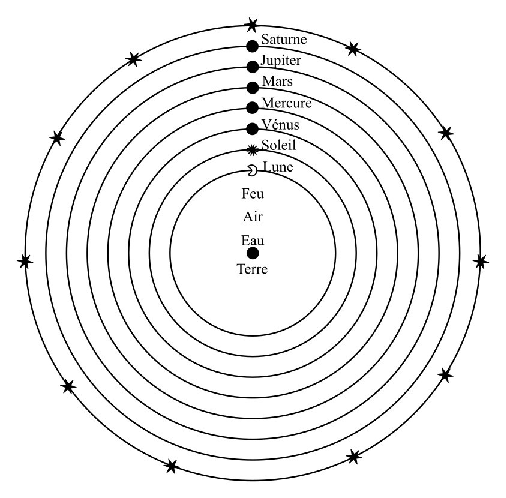
\includegraphics[width=0.4\textwidth,height=\textheight]{figures/grav/geo.pdf}

}

\caption{Le modèle géocentrique}

\end{figure}%

Cependant, ce modèle est très vite confronté à certaines difficultés.
L'une d'elles concerne le mouvement de Mars autour de la Terre.

\begin{figure}[H]

{\centering 
\includegraphics[width=0.2\textwidth,height=\textheight]{figures/grav/mars.pdf}

}

\caption{QR-code: Orbite de Mars autour de la Terre}

\end{figure}%

Tu peux observer sur l'animation ci-dessus que Mars a un mouvement
rétrograde autour de la Terre. Cette observation était déjà réalisée
plus de deux siècles avant Jésus-Christ, et deux savants de l'époque,
Apollonius et Hipparque, ont tenté d'expliquer pourquoi Mars a un tel
mouvement : ils ont mis au point les premiers modèles par épicycles. Ces
modèles décrivent le mouvement de Mars (mais aussi d'autres astres) de
la manière suivante : Mars se déplace le long d'un cercle, à vitesse
constante, et le centre de ce cercle se déplace lui-même sur un grand
cercle dont le centre est la Terre.

\begin{figure}[H]

{\centering 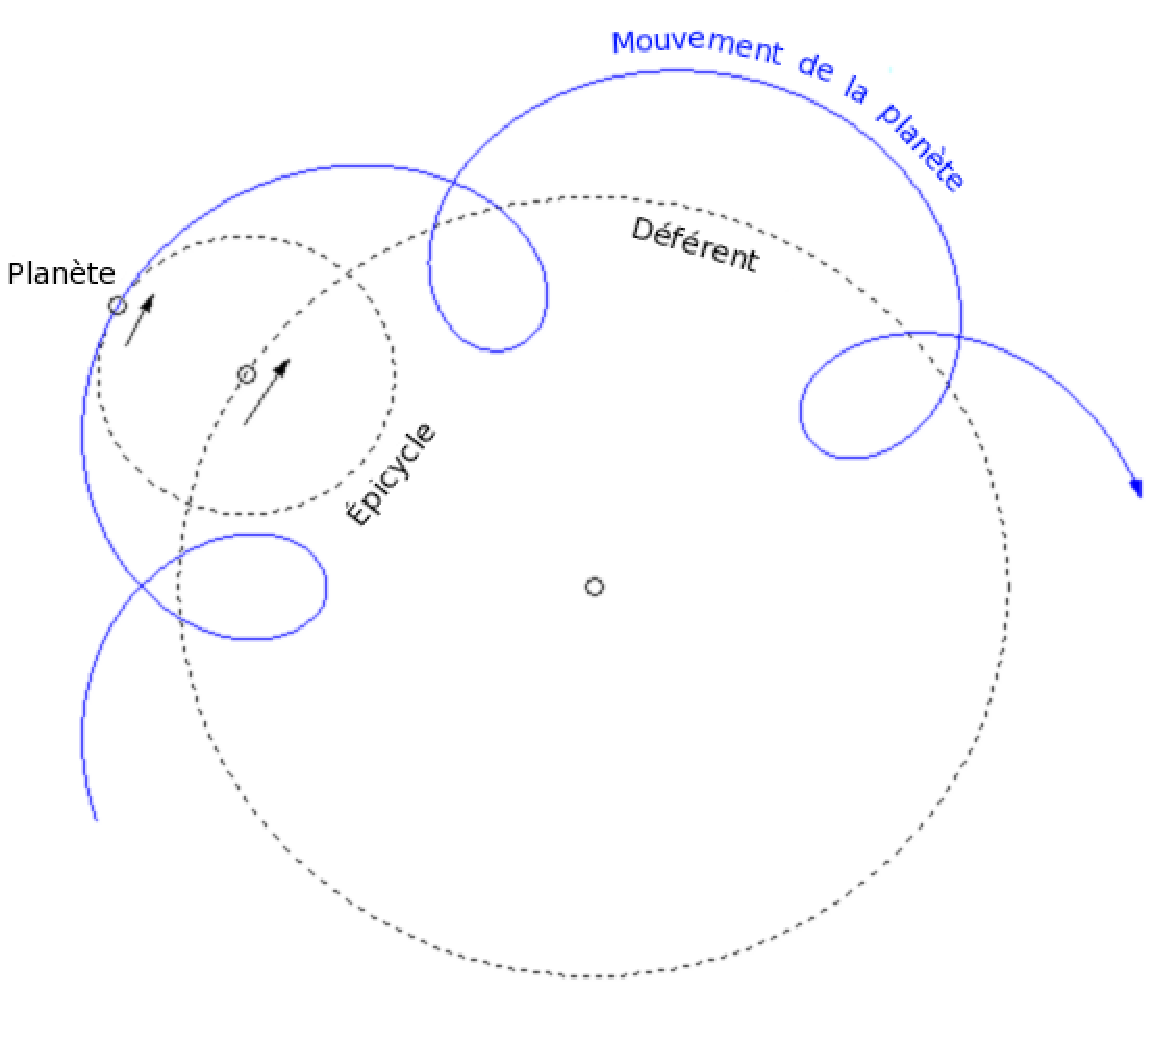
\includegraphics[width=0.4\textwidth,height=\textheight]{figures/grav/epicycle.pdf}

}

\caption{Modèle géocentrique avec épicycle}

\end{figure}%

Ces modèles par épicycles ont été étudiés et raffinés pendant longtemps,
pour aboutir au modèle de Ptolémée, qui proposa un modèle avec plusieurs
épicycles pour expliquer les défauts de mesure des modèles d'Apollonius
et Hipparque. Les travaux de Ptolémée furent la référence en astronomie
jusqu'au XVIe siècle, avec l'arrivée du modèle héliocentrique de
Copernic.

\subsection{Les modèles
héliocentriques}\label{les-moduxe8les-huxe9liocentriques}

Malgré la précision importante des modèles géocentriques, les astronomes
du XVIe siècle n'arrivent pas à prévoir parfaitement le mouvement des
astres. Copernic émit l'hypothèse que le Soleil était au centre de
l'Univers et que la Terre effectue un mouvement circulaire autour de lui
: c'est la naissance des modèles héliocentriques. Bien que le modèle
héliocentrique de Copernic représente une révolution en astronomie, il
ne permet pas une plus grande précision dans les prédictions que dans le
modèle de Ptolémée. La raison est que Copernic suppose que les astres
décrivent des cercles autour du Soleil.

\begin{figure}[H]

{\centering 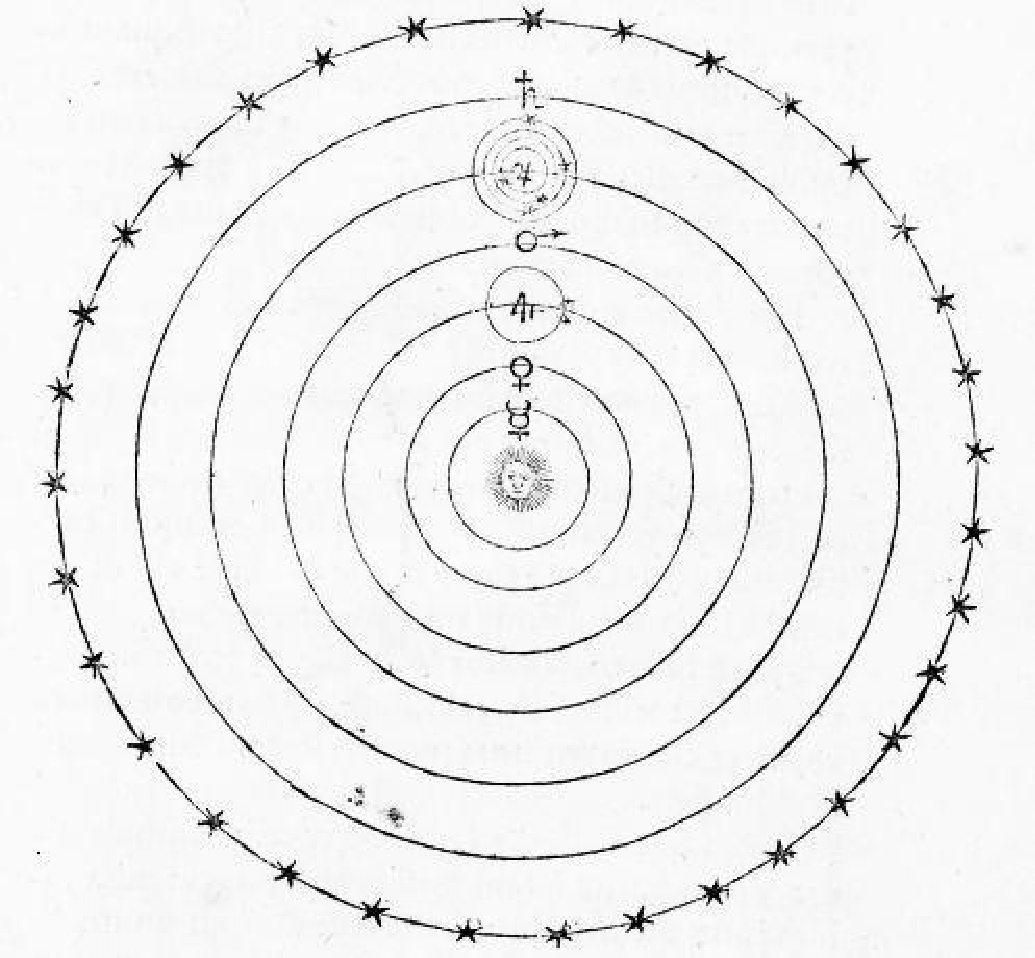
\includegraphics[width=0.4\textwidth,height=\textheight]{figures/grav/copernic.pdf}

}

\caption{Le modèle de Copernic}

\end{figure}%

Cependant, un atout du modèle de Copernic est sa simplicité par rapport
au modèle avec épicycles. De plus, le mouvement rétrograde de Mars
s'explique facilement comme un effet de perspective d'un observateur sur
Terre.

\begin{figure}[H]

{\centering 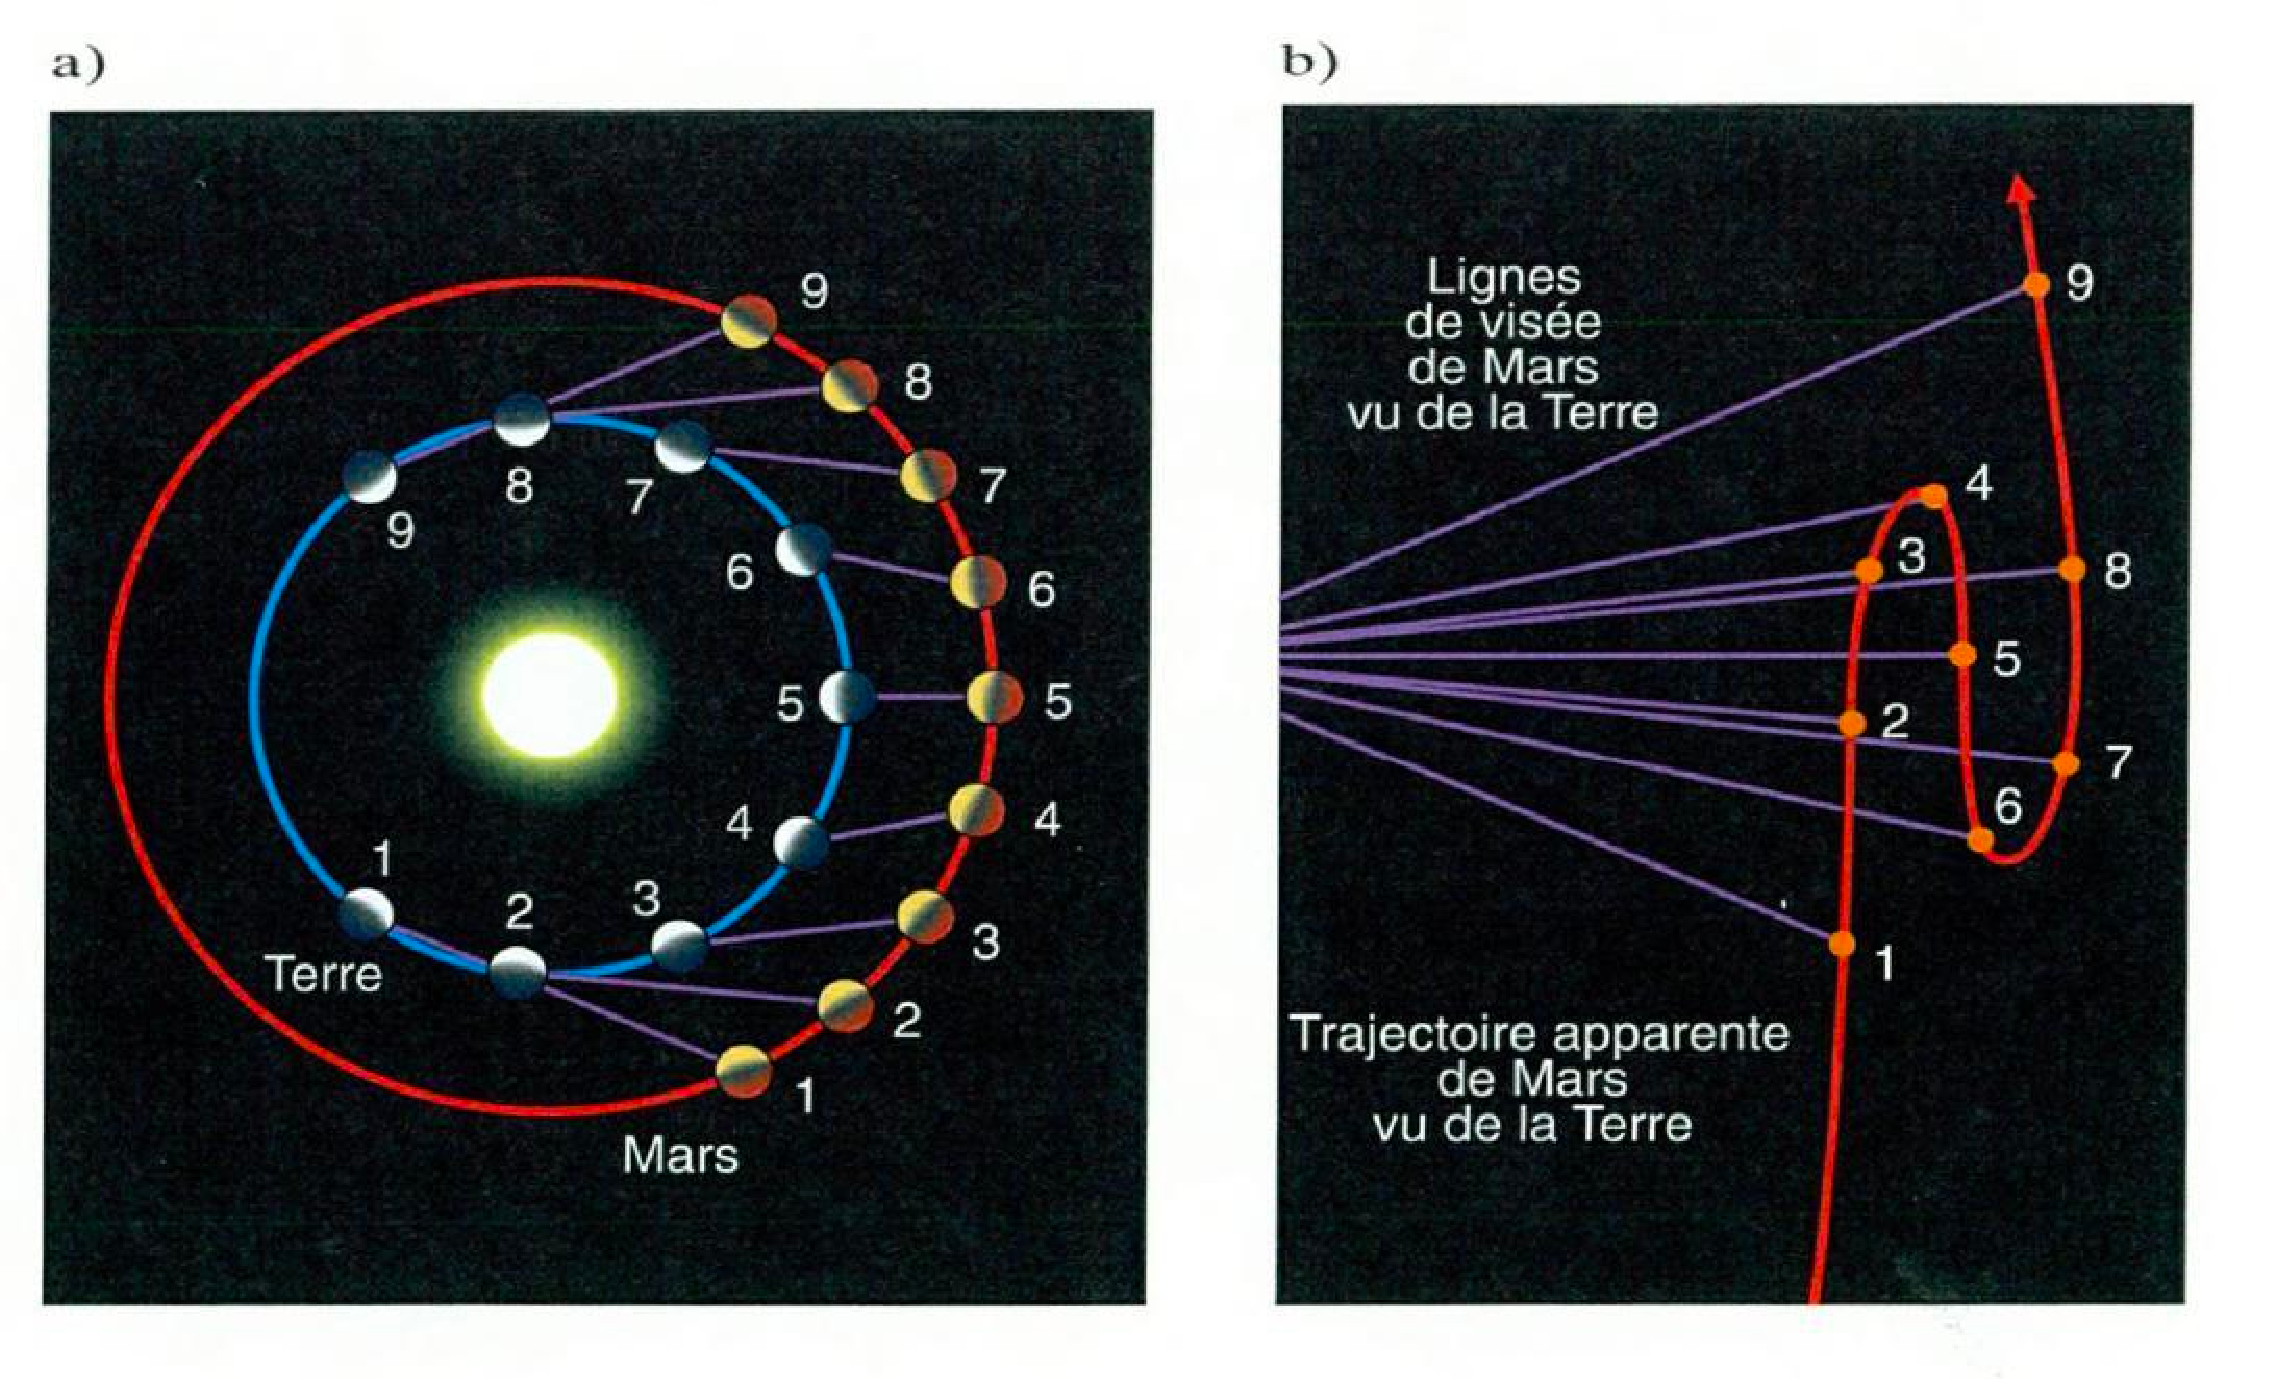
\includegraphics[width=1\textwidth,height=\textheight]{figures/grav/mars-2.pdf}

}

\caption{Orbite de Mars dans le modèle héliocentrique}

\end{figure}%

Le modèle de Copernic ne rencontrera pas un franc succès auprès de ses
contemporains : ceux-ci étaient, entre autres, influencés par le sens
commun de l'époque et les dogmes religieux.\\
Au XVIIe siècle, Galilée se positionne en défenseur du modèle de
Copernic : il apporta des arguments importants en faveur de ce modèle,
grâce à des observations des satellites de Jupiter faites avec une
lunette astronomique. Il observe que Jupiter et ses satellites forment
un système planétaire miniature autour d'un centre qui n'est pas la
Terre.

\subsection{Les lois de Kepler}\label{les-lois-de-kepler}

Le modèle de Copernic place le Soleil au centre de l'Univers et suppose
que les astres décrivent un mouvement circulaire dont le centre est le
Soleil. Cependant, les mesures des mouvements des astres ne collent pas
parfaitement aux trajectoires du modèle et Copernic fait vite appel aux
épicycles pour améliorer son modèle. Malgré ces améliorations, le modèle
héliocentrique reste imparfait.

C'est à la fin du XVIe siècle qu'une avancée majeure est réalisée pour
expliquer le mouvement des astres : Johannes Kepler, sur base de mesures
méticuleuses réalisées par l'astronome danois Tycho Brahe, se rend
compte que les planètes ne décrivent pas des mouvements circulaires mais
elliptiques, dont un des foyers est occupé par le Soleil. Il s'agit de
sa première loi, parmi trois qui tentent de décrire le mouvement des
planètes autour du Soleil.

\begin{tcolorbox}[enhanced jigsaw, rightrule=.15mm, colframe=quarto-callout-note-color-frame, arc=.35mm, opacityback=0, leftrule=.75mm, bottomrule=.15mm, breakable, left=2mm, toprule=.15mm, colback=white]
\begin{minipage}[t]{5.5mm}
\textcolor{quarto-callout-note-color}{\faInfo}
\end{minipage}%
\begin{minipage}[t]{\textwidth - 5.5mm}

\vspace{-3mm}\textbf{Première loi: la loi des orbites.}\vspace{3mm}

La trajectoire de chaque planète est une ellipse dont un foyer est
occupé par le Soleil.

\end{minipage}%
\end{tcolorbox}

\begin{figure}[H]

{\centering 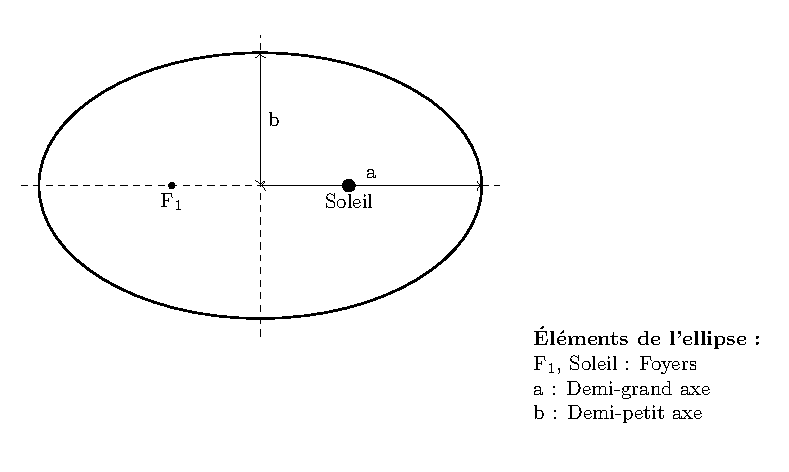
\includegraphics[width=0.8\textwidth,height=\textheight]{figures/grav/fig1.pdf}

}

\caption{Trajectoire elliptique}

\end{figure}%

\begin{tcolorbox}[enhanced jigsaw, rightrule=.15mm, colframe=quarto-callout-note-color-frame, arc=.35mm, opacityback=0, leftrule=.75mm, bottomrule=.15mm, breakable, left=2mm, toprule=.15mm, colback=white]
\begin{minipage}[t]{5.5mm}
\textcolor{quarto-callout-note-color}{\faInfo}
\end{minipage}%
\begin{minipage}[t]{\textwidth - 5.5mm}

\vspace{-3mm}\textbf{Deuxième loi: loi des aires.}\vspace{3mm}

Le segment qui joint le Soleil à une planète balaie des secteurs d'aires
égales en des durées égales, quelles que soient ces durées.

\end{minipage}%
\end{tcolorbox}

\begin{figure}[H]

{\centering 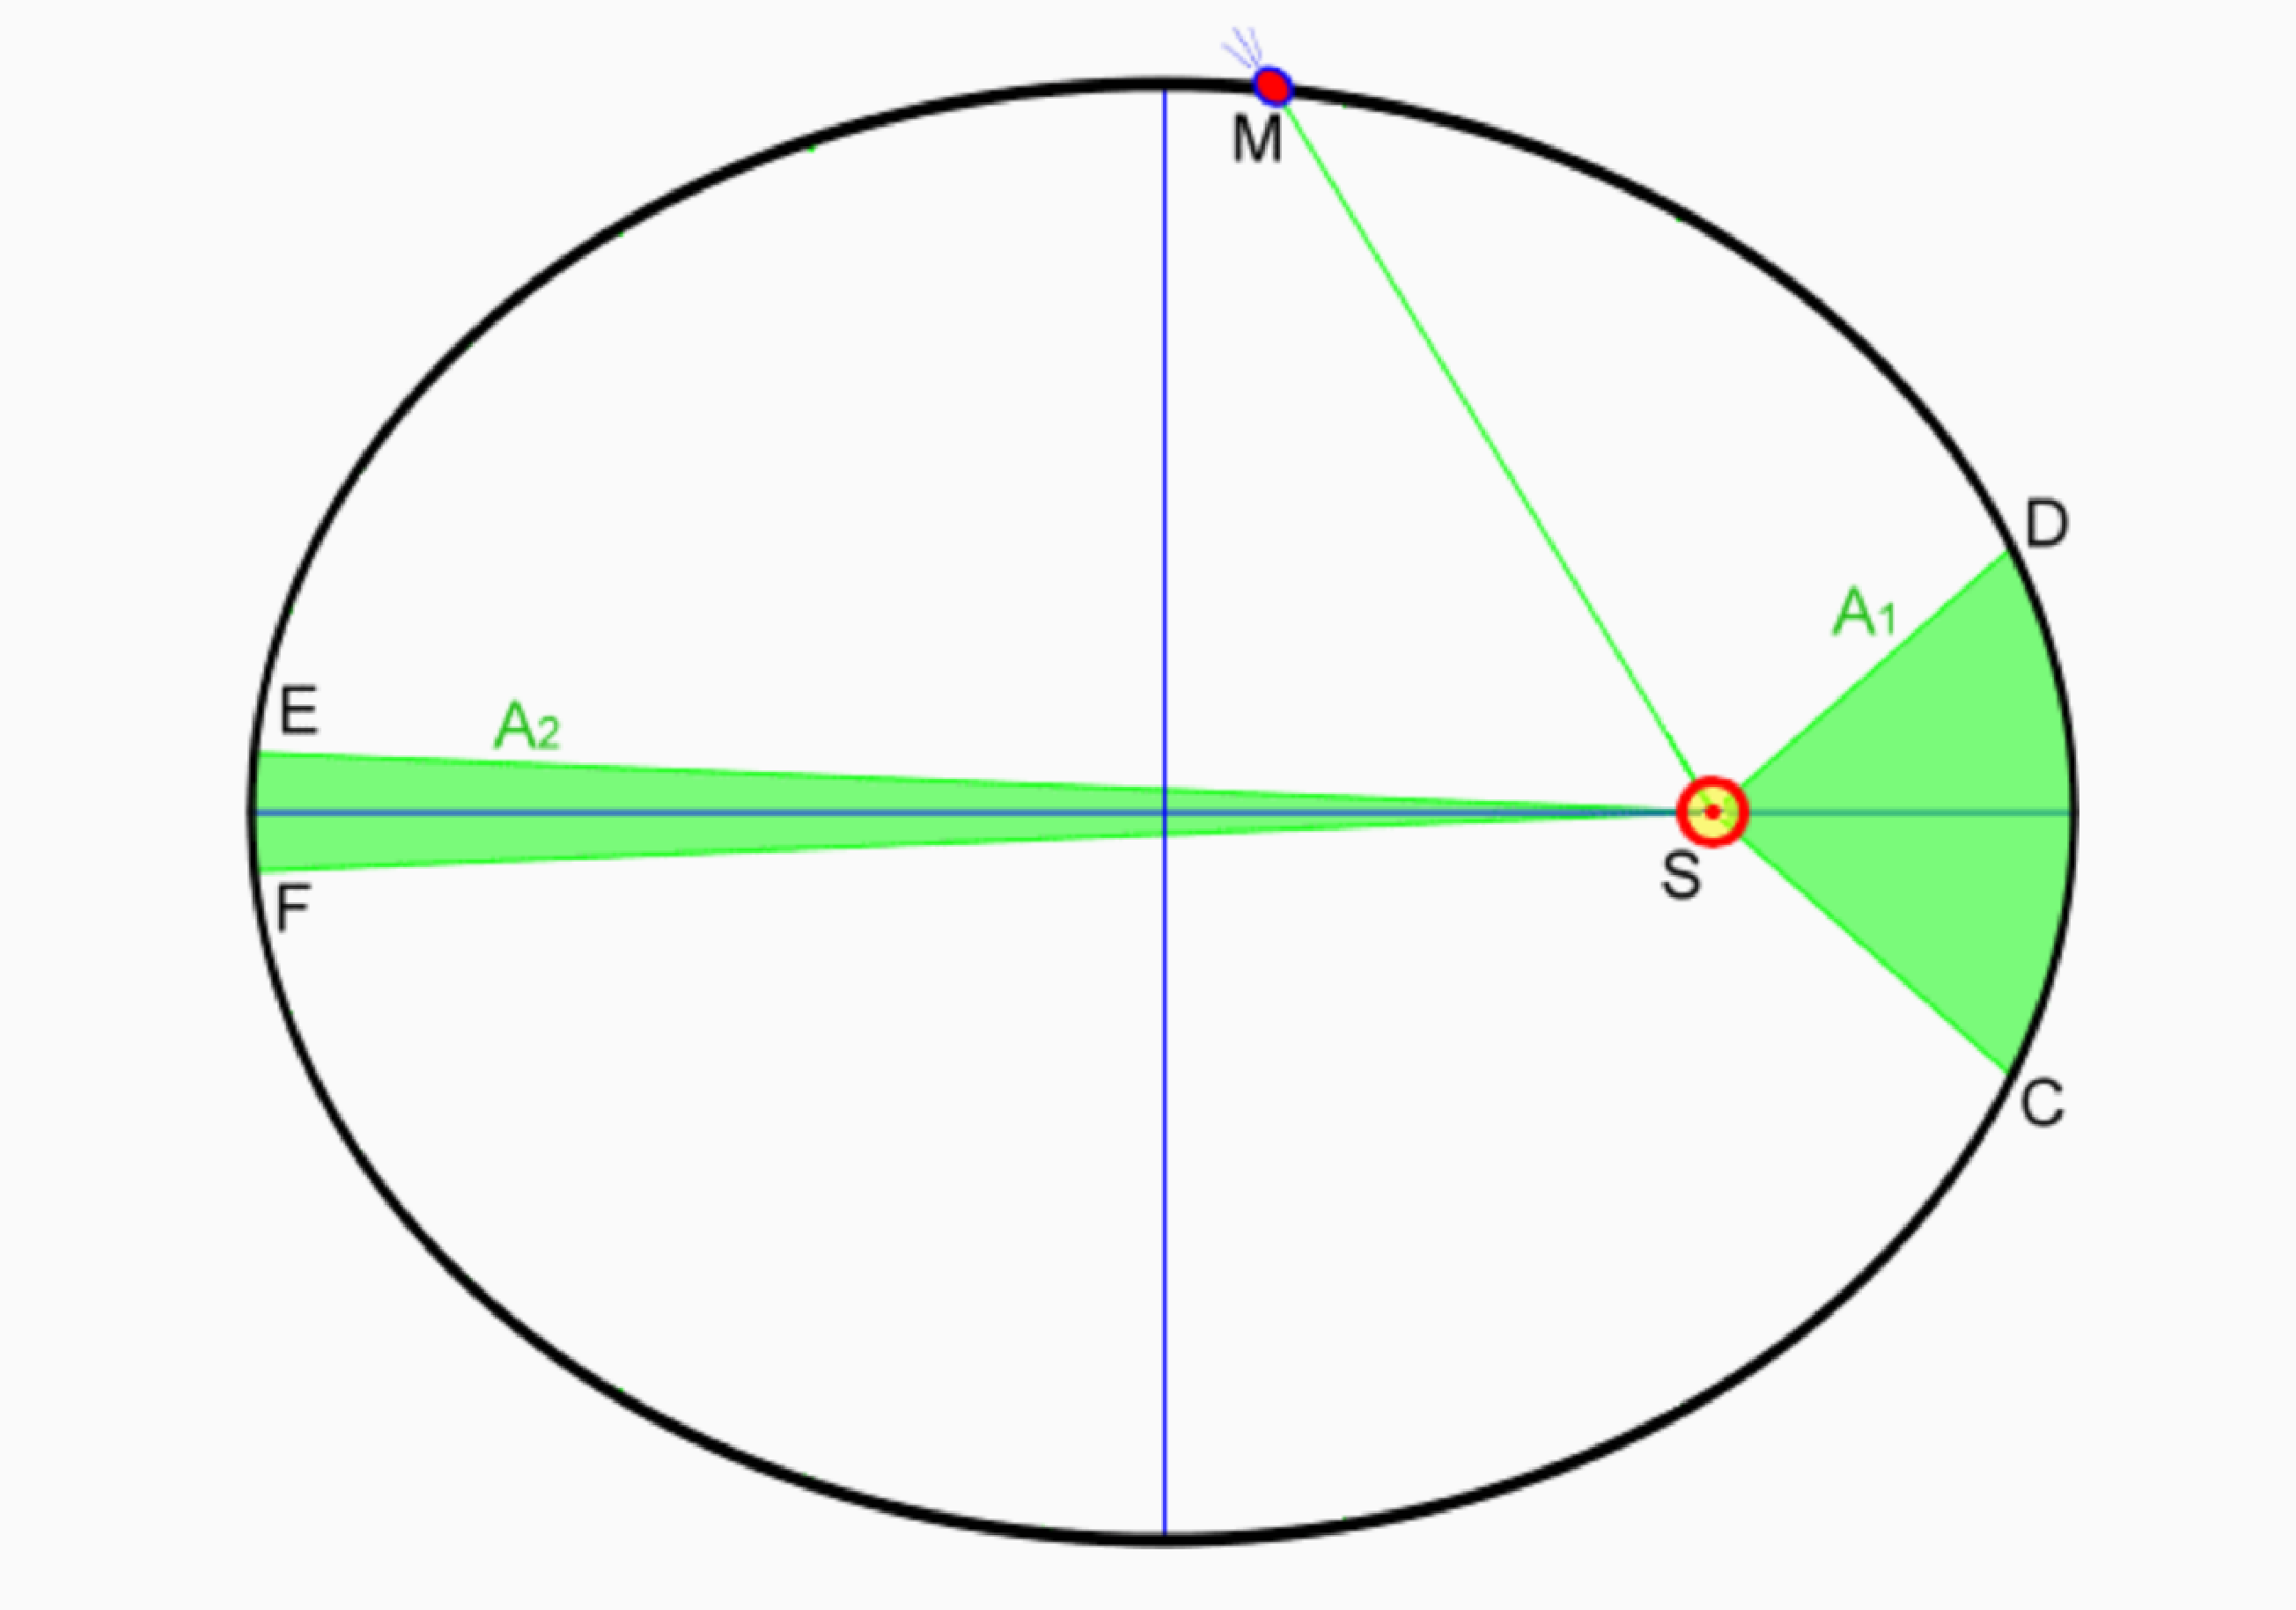
\includegraphics[width=0.8\textwidth,height=\textheight]{figures/grav/aires.pdf}

}

\caption{Loi des aires}

\end{figure}%

\begin{tcolorbox}[enhanced jigsaw, rightrule=.15mm, colframe=quarto-callout-note-color-frame, arc=.35mm, opacityback=0, leftrule=.75mm, bottomrule=.15mm, breakable, left=2mm, toprule=.15mm, colback=white]
\begin{minipage}[t]{5.5mm}
\textcolor{quarto-callout-note-color}{\faInfo}
\end{minipage}%
\begin{minipage}[t]{\textwidth - 5.5mm}

\vspace{-3mm}\textbf{Troisième loi: loi des périodes.}\vspace{3mm}

Le quotient du cube du demi-grand axe par le carré de la période de
révolution est le même pour toutes les planètes : \[
\frac{a^3_1}{T_1^2}=\frac{a^3_2}{T_2^2}=\ldots
\]

\end{minipage}%
\end{tcolorbox}

\begin{exercise}[]\protect\hypertarget{exr-kepler}{}\label{exr-kepler}

Complète le tableau suivant à l'aide de la 3e loi de Kepler.

\begin{longtable}[]{@{}
  >{\raggedright\arraybackslash}p{(\columnwidth - 6\tabcolsep) * \real{0.3100}}
  >{\raggedright\arraybackslash}p{(\columnwidth - 6\tabcolsep) * \real{0.2300}}
  >{\raggedright\arraybackslash}p{(\columnwidth - 6\tabcolsep) * \real{0.2300}}
  >{\raggedright\arraybackslash}p{(\columnwidth - 6\tabcolsep) * \real{0.2300}}@{}}
\toprule\noalign{}
\begin{minipage}[b]{\linewidth}\raggedright
Planète
\end{minipage} & \begin{minipage}[b]{\linewidth}\raggedright
\(a(10^9\text{m})\)
\end{minipage} & \begin{minipage}[b]{\linewidth}\raggedright
\(T(10^6\text{s})\)
\end{minipage} & \begin{minipage}[b]{\linewidth}\raggedright
\(a^3/T^3(10^{15}\text{m}^3/\text{s}^2)\)
\end{minipage} \\
\midrule\noalign{}
\endhead
\bottomrule\noalign{}
\endlastfoot
Mercure & 57,9 & & 3356 \\
Vénus & 108,1 & 19,41 & \\
Terre & 149,6 & & \\
Mars & & 59,36 & 3364 \\
Jupiter & 778,4 & 374,3 & \\
Saturne & 1424 & 928,4 & \\
\end{longtable}

\end{exercise}

\subsection{La loi de la gravitation
universelle}\label{la-loi-de-la-gravitation-universelle}

Kepler a décrit avec précision le mouvement des planètes, mais il ne l'a
pas expliqué. Il faut attendre le XVIIe siècle et Isaac Newton pour
comprendre pourquoi les planètes suivent ces trajectoires elliptiques.

Newton propose que toutes les masses s'attirent mutuellement avec une
force qui dépend de certaines de leurs carctéristiques. Il va montrer
ainsi que l'interaction qui fait tomber un objet sur Terre est aussi
responsable du mouvement des planètes autour du Soleil. Cette idée
révolutionnaire unifie les phénomènes terrestres et célestes sous une
même loi.

Cette loi permet non seulement d'expliquer les trajectoires des planètes
décrites par Kepler, mais aussi d'autres phénomènes tels que la chute
des objets sur Terre, les marées ou encore le mouvement des satellites
artificiels.

Newton montre que les lois de Kepler sont une conséquence directe de la
gravitation universelle : en appliquant ses lois du mouvement et la
force gravitationnelle, il retrouve les trajectoires elliptiques des
planètes. C'est ainsi que la physique moderne voit le jour : un même
principe explique à la fois le mouvement des planètes et celui des
objets terrestres.




\end{document}
